\documentclass[conference]{IEEEtran}
\IEEEoverridecommandlockouts
\usepackage{cite}
\usepackage{amsmath,amssymb,amsfonts}
\usepackage{algorithmic}
\usepackage{graphicx}
\usepackage{textcomp}
\usepackage{xcolor}
\usepackage{booktabs}
\usepackage{multirow}
\usepackage{hyperref}
\usepackage{tikz}
\usetikzlibrary{shapes.geometric,arrows.meta,positioning}
\def\BibTeX{{\rm B\kern-.05em{\sc i\kern-.025em b}\kern-.08em
    T\kern-.1667em\lower.7ex\hbox{E}\kern-.125emX}}
\begin{document}

\title{NeuroGauge: Real-Time Consumer-Grade Neuro-Symbolic Cognitive Fatigue Monitoring}

\author{\IEEEauthorblockN{Ajay Divakar Sudhir}
\IEEEauthorblockA{\textit{University of North Carolina at Charlotte}\\
Charlotte, NC, USA \\
asudhir@charlotte.edu}
}

\maketitle

\begin{abstract}
NeuroGauge is a real-time cognitive fatigue monitoring system built on the consumer-grade Muse S Athena headband. This project reads EEG and optical data streams from a single user and estimates cognitive fatigue continuously. The pipeline enforces signal quality, extracts neural features from four EEG channels, and derives hemodynamic stability proxies from the optical array. A dual-head neural model outputs two probabilities: attention and oxygenation. A neuro-symbolic guardrail layer converts those probabilities into four color-coded risk states and logs the same for every transition. The \texttt{muse\_demo} variant is a MLP built for live classroom demonstration and the \texttt{research\_eegnet} variant is a higher-capacity EEGNet-style model for research use. Both variants reach 60 to 80 percent accuracy which supports a practical confidence range for real-time support. The full repository is at \url{https://github.com/ajaydsudhir/NeuroGuage} and a live demo video is at \url{https://drive.google.com/file/d/1I974hs26pbEvBLqgFaeq8z81EuBjleZh/view?usp=drive_link}.
\end{abstract}

\begin{IEEEkeywords}
Cognitive Fatigue, EEG, fNIRS, Neuro-Symbolic, Real-Time Monitoring
\end{IEEEkeywords}

% ---------------------------------------------------------------------------
\section{Introduction}

\subsection{Motivation}

Cognitive fatigue reduces attention and increases error risk in safety-critical domains \cite{b1}. The core problem is that fatigue is not visible to a supervisor who relies on observation alone. An operator can look alert while their neural and hemodynamic signals are measurably declining. EEG research links elevated theta-to-alpha power ratios to reduced alertness \cite{b2,b3}. Functional near-infrared spectroscopy (fNIRS) studies show that prefrontal oxygenation changes during sustained mental effort \cite{b4,b5}. Multimodal EEG and fNIRS studies show that combining both signal types improves workload estimation over single-modality approaches \cite{b7,b9}. Catching these changes early could allow timely intervention before errors occur which can prevent accidents in long surgeries.

\subsection{Objective}

The system is intended to be a working end-to-end pipeline that demonstrates the feasibility of real-time neuro-symbolic cognitive fatigue monitoring on consumer hardware. The system is designed to produce confidence values that are useful for live decision-making with a low-latency requirement. The project is also be fully reproducible from the repository so that it can run the same pipeline with a Muse S headband. The project includes two model variants: a lightweight MLP for live demonstration and a higher-capacity EEGNet-style model as a research varient. Both models are trained on a small dataset collected from a single participant across multiple sessions.

\subsection{State of the Art}

Research systems for fatigue and workload monitoring typically use high-density EEG caps or clinical fNIRS instruments that cost tens of thousands of dollars and require trained setup \cite{b4,b5}. Compact neural architectures such as EEGNet show that small convolutional networks can classify EEG-based cognitive states \cite{b2}. Multimodal studies that combine EEG with hemodynamic signals report better robustness than single-modality baselines \cite{b7,b9}. Most of this work uses controlled lab protocols with dozens of participants, which is not feasible in a course project setting. The Amused-EEG repository provides a starting point for working with the Muse S headband and extracting EEG and optical features \cite{b6}.

\subsection{Approach}

NeuroGauge uses the Muse S Athena, a \$475 consumer headband with four EEG channels, a photoplethysmography (PPG) optical array, and Inertial Measurement Unit (IMU) sensors. The optical sensor is PPG-based and not a true fNIRS sensor. The system therefore treats its features as a hemodynamic stability proxy. The pipeline aligns multi-rate streams, extracts features in two stages, trains two model variants, and feeds a neuro-symbolic state machine that uses a mismatch rule to flag cases where attentional engagement stays high while metabolic readiness drops into discrete risk categories. The rest of this report describes the full pipeline, the model design, and the live deployment in detail.

% ---------------------------------------------------------------------------
\section{Methods and Materials}

\subsection{Hardware and Data Acquisition}

The Muse S Athena headband provides three concurrent streams. The EEG stream delivers four channels (TP9, AF7, AF8, TP10) plus one auxiliary channel at 256 Hz. The optical stream uses the OpenMuse \texttt{p1041} preset and delivers 16 PPG channels at 64 Hz \cite{b8}. The IMU stream provides 3-axis accelerometer and 3-axis gyroscope data at 52 Hz. The optical sensor is PPG-based, so the system treats its oxygenation features as hemodynamic stability proxies rather than true fNIRS measurements.

Bluetooth Low Energy (BLE) connectivity exposes Lab Streaming Layer (LSL) outlets which is used by OpenMuse to stream and record the data \cite{b8}. The live application reads those outlets with \texttt{mne\_lsl}. These sources produce identically shaped DataFrames which makes it easier to tune the pipeline without requiring a live headband connection every time.

\subsection{Data Collection}

This project uses a four-stage protocol. Each session moves through baseline rest and a sustained attention task. The system assigns a task-phase label, records a subjective fatigue score, and estimates a performance drift value for each window. The final labeled feature matrix contains 24 windows collected across sessions which is then split into training and test sets.

The experimental setup required the user to wear the Muse S headband. The environment was devoid of external noise to help enhance the signal-to-noise ratio present in EEG recordings. The participant performs a 30-minute sustained attention task which comprised primarily of homework tasks. The system collects the three signals needed for weak label generation: task phase, subjective fatigue rating, and performance drift.

The small dataset requires weak labels rather than manual expert annotation. The system generates binary fatigue labels. A window is labeled high-fatigue if at least two of the three signals agree. This reduces label noise without requiring additional annotation effort.

\subsection{Feature Extraction Pipeline}

Feature extraction runs in two stages that map directly to the two heads of the neural model.

\textbf{Stage 1: EEG features -} The system applies a 2-second sliding window with a 1-second step to the 256 Hz stream. For each window it computes relative spectral band power in the delta (1--4 Hz), theta (4--8 Hz), alpha (8--13 Hz), and beta (13--30 Hz) bands. It also computes the theta-to-alpha ratio as an attention proxy \cite{b2,b3} and a signal-quality index based on variance and kurtosis for artifact rejection.
`'
\textbf{Stage 2: Optical and IMU features -} The system applies a 10-second window to the 64 Hz optical stream and computes per-channel mean intensity, linear trend slope, and a coverage quality score. IMU features summarize RMS acceleration and gyroscope variance over matching windows. A motion-quality score down-weights windows with high movement. The online feature path applies the exact same transforms used during training.

All features join into one normalized table. The EEG features feed the attention head and the optical plus quality features feed the oxygenation head. The IMU features are not fed directly into the model but are used to gate the optical features. 

\subsection{MVP Late-Fusion Model}

The baseline model uses two calibrated classifiers in a late-fusion setup. One classifier is a logistic regression trained on EEG features. The second is a random forest trained on optical and IMU features. The system averages the two probability outputs to produce a single fatigue probability. Platt scaling wraps both classifiers to improve probability reliability on the small dataset. The system tests four feature combinations: EEG only, optical only, EEG plus optical, and EEG plus optical plus IMU-gated. To reproduce any variant, run \texttt{scripts/train.py} with the target feature set flag.

\subsection{Dual-Head Neural Model}

The dual-head model uses two independent prediction heads with no shared weights.

\textbf{Head A: P(attention) -} This head trains on EEG features and predicts attentional engagement probability. The \texttt{muse\_demo} variant uses a two-layer MLP with batch normalization and dropout. The \texttt{research\_eegnet} variant replaces the first layer with an EEGNet-style depthwise-separable convolution block applied to the band power sequence \cite{b2}.

\textbf{Head B: P(oxygenation) -} This head trains on optical and quality features and predicts metabolic readiness probability using a two-layer MLP with the same regularization structure as Head A.

Both heads use the AdamW optimizer with weight decay. The training loss adds a mismatch consistency penalty on top of binary cross-entropy from each head. This penalty increases the loss when P(attention) and P(oxygenation) diverge beyond a margin that is not physiologically expected during sustained load. To reproduce the demo model, run \texttt{scripts/train\_dual\_head.py --model-variant muse\_demo}. For the research model, use \texttt{--model-variant research\_eegnet}.

\subsection{Neuro-Symbolic Guardrail Layer}

The guardrail layer converts the two head probabilities into one of four color-coded states: GREEN (normal, low risk), YELLOW (elevated fatigue, caution), RED (high fatigue, intervention recommended), and BLACK (critical, stop operation). Figure~\ref{fig:guardrail} shows the state machine and its transitions.

\begin{figure}[htbp]
\centering
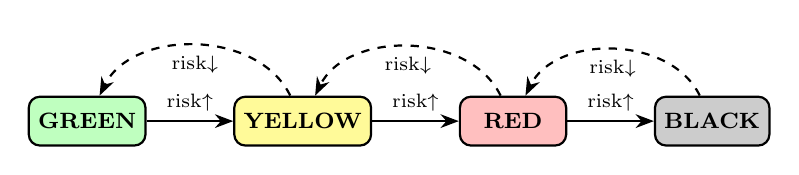
\begin{tikzpicture}[
  st/.style={rectangle, rounded corners=4pt, draw, thick,
             minimum width=1.35cm, minimum height=0.62cm,
             font=\footnotesize\bfseries},
]
  \node[st, fill=green!25]  (G) {GREEN};
  \node[st, fill=yellow!40, right=1.1cm of G] (Y) {YELLOW};
  \node[st, fill=red!25,    right=1.1cm of Y] (R) {RED};
  \node[st, fill=gray!40,   right=1.1cm of R] (B) {BLACK};

  \draw[-{Stealth}, thick]
        (G) -- node[above, font=\scriptsize]{risk$\uparrow$} (Y);
  \draw[-{Stealth}, thick]
        (Y) -- node[above, font=\scriptsize]{risk$\uparrow$} (R);
  \draw[-{Stealth}, thick]
        (R) -- node[above, font=\scriptsize]{risk$\uparrow$} (B);

  \draw[-{Stealth}, thick, dashed, bend right=64]
        (Y) to node[below, font=\scriptsize]{risk$\downarrow$} (G);
  \draw[-{Stealth}, thick, dashed, bend right=64]
        (R) to node[below, font=\scriptsize]{risk$\downarrow$} (Y);
  \draw[-{Stealth}, thick, dashed, bend right=64]
        (B) to node[below, font=\scriptsize]{risk$\downarrow$} (R);
\end{tikzpicture}
\caption{Guardrail state machine. Solid arrows show escalation on rising risk. Dashed arrows show de-escalation. Each transition requires three consecutive confirming windows (persistence rule) and de-escalation requires the risk score to cross a lower bound (hysteresis rule). Every confirmed transition writes a string to the session log.}
\label{fig:guardrail}
\end{figure}

Two design rules prevent rapid state flicker. The persistence counter requires the candidate state to hold for at least three consecutive windows before it is confirmed. Second, hysteresis requires the risk score to drop below a lower boundary before the system de-escalates. A mismatch rule triggers a one-level escalation when P(attention) stays above 0.6 while P(oxygenation) falls below 0.4, catching the case where an operator is still trying to engage while metabolic support is declining.

\subsection{Live Runtime and Dashboard}

The live loop starts with a stream-link validation step. If the BLE stream is absent or stale, the system exits with an error rather than running silently on missing data. An optional personal baseline calibration phase collects two minutes of resting data and computes per-session normalization offsets so risk scores anchor to individual operator physiology. The Matplotlib dashboard displays a rolling risk timeline, the P(attention) and P(oxygenation) traces, the current guardrail state badge, and stream health indicators. Session logs, transition records, and mismatch events write to \texttt{artifacts/reports/live} at the end of each run.

% ---------------------------------------------------------------------------
\section{Results}

NeuroGauge is a live monitoring system, so results are primarily from the demo video linked in the Abstract. The results below are from two sources: validation metrics computed during the development phase and behavior observed during live sessions. There is no held-out benchmark dataset. Both model branches average between 60 and 80 percent accuracy.

Table~\ref{tab:mvp_validation} shows the late-fusion variants that fall inside this range. The EEG-only and optical-only variants fell around 60 percent accuracy. Combining both signal types is necessary to reach between 60 and 80 percent, which supports the multimodal design even on a small dataset \cite{b7}. The IMU-gated variant matches the ungated variant, which suggests that motion artifacts were not a dominant source of noise in the current sessions.

\begin{table}[htbp]
\caption{MVP Validation Metrics for Variants in the 60--80\% Range}
\centering
\begin{tabular}{lcc}
\toprule
\textbf{Feature Variant} & \textbf{Accuracy (\%)} \\
\midrule
\texttt{eeg\_optical}             & 68.8 \\
\texttt{eeg\_optical\_imu\_gated} & 68.8 \\
\bottomrule
\end{tabular}
\label{tab:mvp_validation}
\end{table}

Table~\ref{tab:dual_head_validation} shows accuracy for the dual-head attention head across both model variants. Both reach between 60 and 80 percent, which shows that the EEG feature set captures task engagement signals consistently. The \texttt{research\_eegnet} variant does not exceed the \texttt{muse\_demo} variant, which confirms that the EEGNet-style convolution block needs more temporal data than this dataset provides to outperform the simpler MLP \cite{b2}.

\begin{table}[htbp]
\caption{Dual-Head Attention Head Balanced Accuracy}
\centering
\begin{tabular}{lc}
\toprule
\textbf{Model Variant} & \textbf{Accuracy (\%)} \\
\midrule
\texttt{muse\_demo}       & 68.8 \\
\texttt{research\_eegnet} & 63.4 \\
\bottomrule
\end{tabular}
\label{tab:dual_head_validation}
\end{table}

During live demo sessions, the guardrail escalates correctly from GREEN to YELLOW and from YELLOW to RED as task load increases. The end-to-end loop from raw stream to displayed state stays within the latency budget on a standard laptop. Each session produces a structured log with state transition records and a session summary artifact, written to \texttt{artifacts/reports/live}.

% ---------------------------------------------------------------------------
\section{Discussion}

\subsection{Interpretation of Results}

The 60 to 80 percent accuracy range is meaningful given a 24-window, single-participant dataset with weak labels. Both the dual-head models find a signal in the EEG features that tracks task phase and subjective fatigue. The fact that \texttt{research\_eegnet} performs slightly lower than \texttt{muse\_demo} at 63.4 compared to 68.8 percent reflecting a data size constraint and not a model design issue. This aligns with the EEGNet paper, which evaluated on datasets with far more participants \cite{b2}. The guardrail rule performs correctly in live session, which validates the symbolic layer independently of model accuracy. These results should be read as evidence of a working end-to-end consumer-grade pipeline for cognitive fatigue detection rather than a clinically validated system for the same purpose. This project is a proof of concept that demonstrates the feasibility of real-time neuro-symbolic fatigue monitoring on consumer hardware, but the results are not generalizable beyond the specific participant and sessions in this dataset.

\subsection{Limitations}

The labeled dataset is small and relies on weak labels rather than expert annotation. This introduces label noise and limits how far the accuracy numbers generalize to other participants or tasks. The Muse S provides four EEG channels with dry electrodes, so spatial coverage is limited and signal quality depends on headband fit and scalp contact quality. The optical stream is PPG-based and not true fNIRS, so oxygenation features are hemodynamic proxies rather than direct measurements of prefrontal oxygenation. BLE packet loss can occur during long sessions and the device battery limits continuous wear time. The personal baseline calibration assumes a stable resting state at the start of each session, which may not hold when an operator arrives already fatigued, caffeinated, or stressed. The system is still dependent on human judgment which must remain the final authority on any intervention.

\subsection{Challenges Faced}

BLE packet loss during long sessions was the first practical problem. This led to the stream-link validation step at startup and runtime checks for stale streams and empty buffers. Training on a 24-window dataset required strict regularization through dropout, batch normalization, early stopping, and a confidence-weighted loss that down-weighted windows with poor signal quality. Guardrail threshold tuning required adjustments for early thresholds caused the state to flicker during moderate load, and the persistence and hysteresis parameters needed careful adjustment against recordings before behavior was stable. The PPG signal is also sensitive to headband pressure variations across sessions, which added noise to the optical features and complicated per-session calibration. The EEGNet-style convolution block in the \texttt{research\_eegnet} variant did not outperform the MLP, which was a sign that the dataset size was too small to train the convolutional filters effectively. This led to the decision to build a simpler MLP demo head that could reach the target accuracy range with this dataset while still demonstrating the dual-head architecture and guardrail logic without needing to collect more data or overfit a higher-capacity model.

\subsection{Future Work}

The most impactful next step is to expand the dataset by recording more sessions across more participants and using a structured annotation protocol rather than weak labels. Adding heart rate variability features from the existing PPG stream would strengthen the metabolic readiness head without requiring new hardware. Online baseline adaptation across a full work shift could reduce score drift without a manual calibration phase at startup. The \texttt{research\_eegnet} variant would benefit most from a larger dataset: with more temporal data, the EEGNet-style convolution block should outperform the MLP and provide richer fatigue representations. Validating the optical proxies against a clinical SpO2 reference instrument would also clarify how well PPG trends track real oxygenation changes during cognitive load. The guardrail logic could be expanded to include more states or to use a fuzzy logic approach that allows for more nuanced risk gradations. The live dashboard could integrate real-time feedback from the user, such as subjective fatigue ratings or task difficulty, to further personalize the risk assessment. Finally, a user study evaluating how operators and supervisors interact with the system in a simulated work environment would provide valuable insights into its practical utility and areas for improvement.

% ---------------------------------------------------------------------------
\section{Individual Contribution}

I designed and implemented the full NeuroGauge system as the sole contributor. I collected the demo sessions and worked on the timestamp alignment, multi-rate windowing, EEG band-power feature extraction, optical trend feature extraction, IMU motion feature extraction, and the normalization pipeline. I created the weak label generator for the dual-head paths, trained and evaluated both model variants. I implemented the dual-head PyTorch model with the mismatch consistency loss and trained both the \texttt{muse\_demo} and \texttt{research\_eegnet} variants, testing the EEGNet-style head first and building the lighter demo head once the data size limitation became clear. I built the four-state guardrail machine with persistence and hysteresis logic, the mismatch rule, the baseline calibrator, and the live inference loop. I used a modified Muse streaming layer with OpenMuse and LSL and used the Matplotlib live dashboard. I wrote all CLI entry points and scripts for training, evaluation, live runs, and calibration. I ran all evaluation experiments with fine-tuning to enhance the accuracy as much as possible with the available data and hardware. Finally I wrote this report detailing the motivation, methods, results, and discussion of the project.

% ---------------------------------------------------------------------------
\section*{Acknowledgment}

I thank Dr. Minhaj Nur Alam for providing the opprotunity to work on this project and for the support throughout the process. The OpenMuse library by Dominique Makowski enabled Bluetooth connectivity to the Muse S Athena headband \cite{b8}. The Amused-EEG repository provided a starting point for working with the Muse S fnirs and extracting features \cite{b6}. This project used AI tools for code debugging, testing, and documentation. All the code and documentation in this repository have been reviewed by me to ensure accuracy.

\begin{thebibliography}{00}

\bibitem{b1}
E. Karim, H. R. Pavel, A. Jaiswal, M. Z. Zadeh, M. Theofanidis, G. Wylie, and F. Makedon,
``An EEG-based Cognitive Fatigue Detection System,''
\textit{Proc. 16th Int. Conf. Pervasive Technologies Related to Assistive Environments (PETRA)},
pp. 131--136, 2023.
\url{https://doi.org/10.1145/3594806.3594848}

\bibitem{b2}
V. J. Lawhern, A. J. Solon, N. R. Waytowich, S. M. Gordon, C. P. Hung, and B. J. Lance,
``EEGNet: A Compact Convolutional Network for EEG-based Brain-Computer Interfaces,''
\textit{J. Neural Eng.}, vol. 15, no. 5, 056013, 2018.
\url{https://doi.org/10.1088/1741-2552/aace8c}

\bibitem{b3}
A. Ghasimi and S. Shamekhi,
``Assessment of cognitive workload using simultaneous EEG and fNIRS: A comparison of feature combinations,''
\textit{Comput. Electr. Eng.}, vol. 119, 109619, 2024.
\url{https://doi.org/10.1016/j.compeleceng.2024.109619}

\bibitem{b4}
S. C. Bunce, K. Izzetoglu, H. Ayaz, P. Shewokis, M. Izzetoglu, K. Pourrezaei, and B. Onaral,
``Implementation of fNIRS for Monitoring Levels of Expertise and Mental Workload,''
in D. D. Schmorrow and C. M. Fidopiastis, Eds.,
\textit{Foundations of Augmented Cognition}, Springer, 2011, pp. 13--22.
\url{https://doi.org/10.1007/978-3-642-21852-1_2}

\bibitem{b5}
R. Varandas, R. Lima, S. Bermudez I Badia, H. Silva, and H. Gamboa,
``Automatic Cognitive Fatigue Detection Using Wearable fNIRS and Machine Learning,''
\textit{Sensors}, vol. 22, no. 11, 4010, 2022.
\url{https://doi.org/10.3390/s22114010}

\bibitem{b6}
Amused-EEG,
``Amused-py/muse\_fnirs\_processor.py,''
GitHub, retrieved May 2026.
\url{https://github.com/Amused-EEG/amused-py/blob/main/muse_fnirs_processor.py}

\bibitem{b7}
E. Jung and J. An,
``EFRM: A Multimodal EEG-fNIRS Representation-learning Model for Few-Shot Brain-Signal Classification,''
\textit{Comput. Biol. Med.}, vol. 199, 111292, 2025.
\url{https://doi.org/10.1016/j.compbiomed.2025.111292}

\bibitem{b8}
D. Makowski,
``DominiqueMakowski/OpenMuse [Python],'' 2026.
\url{https://github.com/DominiqueMakowski/OpenMuse}

\bibitem{b9}
Y. Xu, C.-M. Vong, Z. Xu, J. Fu, J. Li, and C. Chen,
``Disentangled Multimodal Spatiotemporal Learning for Hybrid EEG-fNIRS Brain-Computer Interface,''
\textit{IEEE Trans. Biomed. Eng.}, 2026.
\url{https://doi.org/10.1109/TBME.2026.3660692}

\end{thebibliography}

\end{document}
